\setchapterpreamble[u]{%
\dictum[Johann Wolfgang von Goethe]{Es ist nicht genug, zu wissen, man muß auch anwenden; es ist nicht genug, zu wollen, man muß auch tun. \dots}}
\chapter{Aufgabenbeschreibung} \index{Aufgabenbeschreibung}\label{kap:aufgabenbeschreibung}

\section{Abstrakte Beschreibung}

%Beispiele für relationen algebra in latex
%Query \verb$SELECT x.a FROM x,y,z WHERE x.a=y.a OR x.a=z.a$
%$\Pi_{x.a} ((x \Join y)\cup(x \Join z))$.
%$temp1 \leftarrow (customer \times account) $ \\
%$temp2 \leftarrow  \sigma_{(customer.sin = account.sin}(temp1)$ \\
%$basic-cust-accts \leftarrow \Pi_{(name, customer.sin, account-number)} (temp2) $ \\
%$basic-cust-accts \leftarrow \Pi_{(name, customer.sin, account-number)} (\sigma_{customer.sin = account.sin}(customer \times account))$

Es soll eine Abfrageschnittstelle (Query-Schnittstelle) für die bereits vorhandene PLIB\footnote{Parts Library - Implementierung nach ISO-13584}  des Fachbereiches erstellt werden. Die Abfrageschnittstelle soll die Abfragen einer Projektion und Selektion analog zu SQL\footnote{Standard Query Language - Abfragesprache für relationale Datenbanken} ermöglichen. 
Konkret wurden vom Fachbereich folgende Möglichkeiten und Operationen als sinnvoll genannt:
\begin{description}
\item[Projektion] Die Attributbeschränkung gleichsam einer \enquote{Spaltenauwahl} in relationalen Datenbanken. In SQL das \enquote{select} Keyword.   

In Relationenalgebra:
$ergebnis-projektion \leftarrow  \Pi_{(attribut_1, attribut_2... attribut_n)}(plib)$ \\

\item[Selektion] Schränkt eine Suche mittels Prädikaten ein auf passende Tupel, gleichsam einer \enquote{Zeilenauswahl}. In SQL das \enquote{where} Keyword samt Mengenoperatoren, wie z.B. \enquote{UND, ODER, NICHT}.

In Relationenalgebra:
$ergebnis-selektion \leftarrow  \sigma_{(praedikat_1, praedikat_2... prädikat_n})(plib)$ \\

\end{description}
 
Diese Abfrageschnittstelle soll die Standards der ISO 29002-31 sowie für deren Nutzung weitere nötige Standards unterstützen, wie z.B. ISO 29002-10. Diese Schnittstelle soll für Menschen sowie für Maschinen einfach nutz- und lesbar sein und soll technisch auf bereits vorhandenen Abfrageprozeduren der Datenbankebene basieren. Die Implementierung dieser Prozeduren und des Datenbankschemas ist Teil der Arbeit zweier Kommilitonen (Herr Mende und Herr Loth).

\section{Zielsetzung}

Das Hauptziel ist die Machbarkeit und die Integration der ISO-Schnittstelle aufbauend auf die vorhandene PLIB Datenbankimplementierung des Fachbereiches aufzuzeigen. 
Ferner ist mit aktuellen Techniken eine Integration, gleichsam Nutzbarkeit der Abfrage der Datenbank zu ermöglichen. Wichtig ist es, die gegebenen ISO Normen zu unterstützen, um Wiederverwendbarkeit zu gewährleisten. Falls Teile der Implementierung von den ISO Normen abweichen oder die Standards erweitert oder geändert werden, wird darauf mit ausführlicher Erläuterung der Gründe hingewiesen. 

Um das Ziel zu erreichen, soll im Rahmen der Arbeit untersucht werden welche mögliche sinnvollen Anwendungsfälle sich in der Praxis basierend auf den zu unterstützenden ISO Standards ergeben. Dafür ist eine Analyse der Standards nötig, um zu prüfen, wie weit und in welcher Art die Abfragemöglichkeiten analog zu SQL unterstützt werden können. Für die Schnittstelle ist eine prototypische Implementierung zu erstellen. Weiterer Bestandteil der Arbeit ist unter Beachtung der technischen Vorgaben eine Analyse der marktaktuellen technischen Möglichkeiten mit anschließender Beschreibung des Auswahlprozesses der Techniken/Plattformen/Architektur und Programmiersprachen. Die Vor- und Nachteile der einzelnen Optionen des Auswahlprozesses und weitere Nutzungs-, respektive Erweiterungs- und Integrationsmöglichkeiten der entwickelten Schnittstelle sind zu erläutern. 
Die Entwicklung der Software soll nach einem aktuell üblichen Softwareentwicklungsprozess erfolgen. Ein enstprechender Prozess ist auszuwählen und zu dokumentieren. 

\section{Details und Abgrenzung}

Dieses Kapitel beschreibt Details und den Kontext der Aufgabenstellung sowie die Abgrenzung zu weiteren Standards und Abschlussarbeiten anderer Studenten. 

\subsection{Gesamtkontext der PLIB Abschlussarbeiten}

Um einen Überblick zu schaffen in welchem Kontext sich diese Arbeit befindet und den Gesamtzusammenhang zu verstehen, soll hier eine kurze Übersicht über die PLIB Abschlussarbeiten geschaffen werden. 

\begin{figure}[htbp]
	\centering
		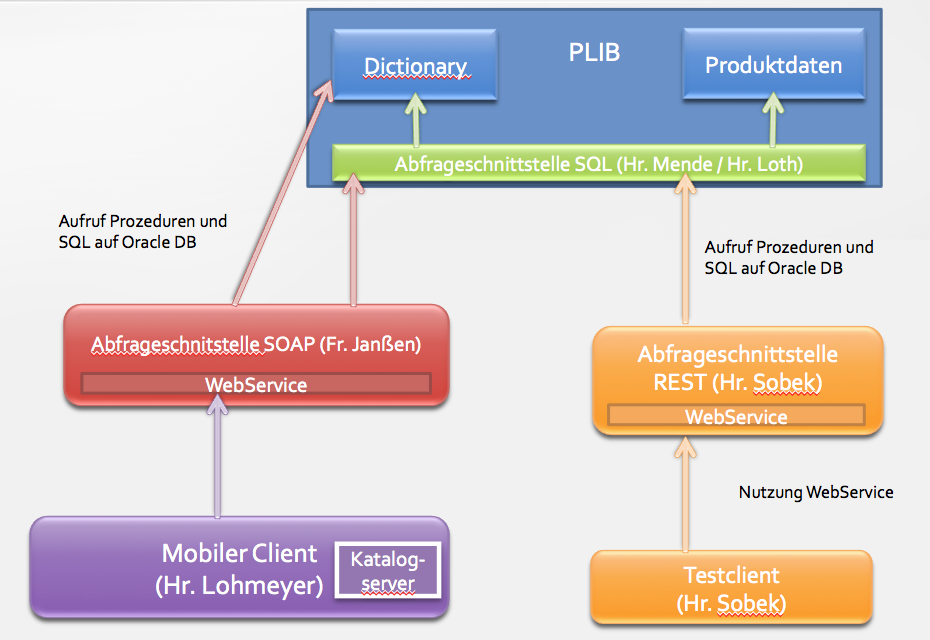
\includegraphics[width=0.98\textwidth]{images/gesamtkontext_plib.png}
	\caption{Gesamtkontext PLIB Abschlussarbeiten}
	\label{fig:gesamtkontext_plib}
\end{figure}

Die Abschlussarbeiten von Herrn Loth und Herrn Mende beziehen sich auf die Umsetzung des PLIB Standards  \citep[Vergl.][]{iso13584-42}.

\subsection{Abgrenzung}

Die Arbeit umfasst die Implementierung der Use Cases nach Kapitel \ref{kap:Use_Cases}. Dies beinhaltet im wesentlichen den Teil 31 der ISO 29002 - einen Abfragestandard für Charakteristische Produktdaten. 
Weiterhin wird für die Datenübertragung eine Implementierung des Teils 10 der ISO 29002 benötigt, siehe Abbildung \ref{fig:lieferketten}. 
Die Arbeit befasst sich nicht mit der Implementierung eines Identification Guides nach ISO 22745-30. Dieser wird in der Praxis von einem Klienten für eine sinnvolle Vorauswahl der für sich oder seine Organisation benötigten Attribute der Teile verwendet. Jeder Klient definiert für seinen Kontext sinnvolle Attribute und Teiledaten und definiert diese mit Hilfe des Schemas der ISO 22745-30. Dies kann mittels eines Webformular auf Klientseite erfolgen oder als allgemeines Formular mit z.B. Excel\footnote{Excel ist ein bekanntes Tabellenkalkulationsprogramm der Firma Microsoft}, welches die für den/die Klienten relevanten Attribute der Produkte enthält die abgefragt werden sollen. Für mehr Informationen zum Identification Guide siehe Kap. \ref{kap:identification_guide}.

%Beispiel: bild mit footnote
\begin{figure}[htbp]
	\centering
		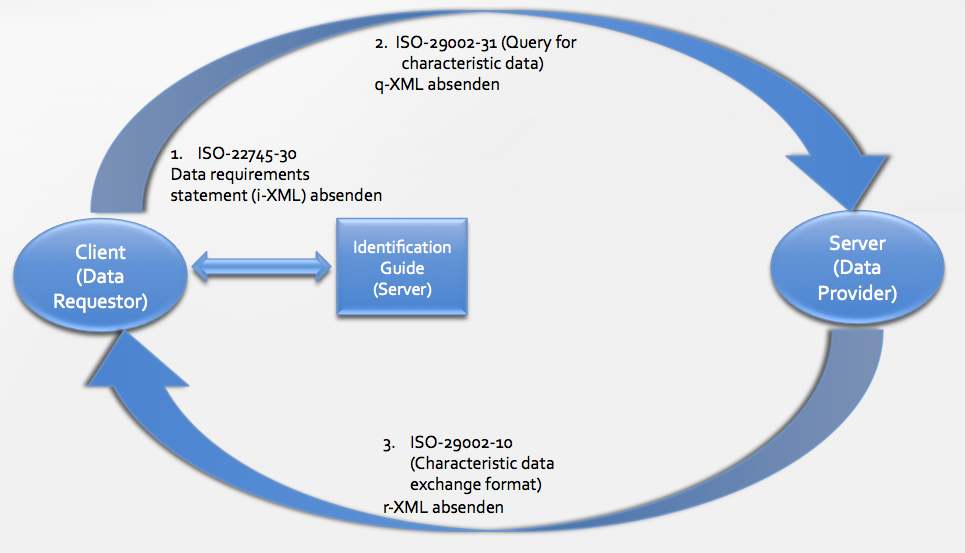
\includegraphics[width=0.99\textwidth]{images/lieferketten_plib.png}
		\caption[Lieferketten]{Lieferketten\footnotemark}
	\label{fig:lieferketten}
\end{figure}
\footnotetext{Abbildung entnommen und abgewandelt aus Benson, Converting Standard Terminology into usable Metadata, 2008 - später in ähnlicher Form auch in Uiterwyk, Die Bedeutung der Merkmalleisten bei eCl@ss, 2012 zu finden.}

\subsection{Vorgaben}

Für die Implementierung sind folgende nichtfunktionale Anforderungen vom Fachbereich vorgegeben:
\begin{description}
\item[Datenbanksystem Oracle] Dieses beinhaltet die PLIB Datenbank samt Abfrageprozeduren und stellt als Teiledatenbank die Basis dar. Dies wird vom Fachbereich bzw. von den Studenten Herr Mende/Herr Loth gestellt. Für die Entwicklung dieses Prototypen wird eine Version von Herrn Mende vom xxx benutzt.  
\item[Web Services] Auf Grund der hohen Verbreitung und Integrationsmöglichkeiten soll die Schnittstelle als Web Service entwickelt werden. Wenngleich die ISO 29002-31 in einem Beispiel eine E-Mail Schnittstelle vorschlägt, ist dies nicht spezifiziert. Siehe Abbildung \ref{fig:datenfluesse}, welche besagt:
\begin{quotation}
Transport: not specified in ISO/TS 29002 (could use email) Payload XML.Query XML schema in ISO/TS 29002-31
\end{quotation}
\item[PLIB Datenbankprozeduren] Die vorhandenen Prozeduren zum Zugriff auf die PLIB Datenbank sollen so weit wie möglich verwendet werden. 
\end{description}

\subsubsection{Technische Beschreibung}
Es soll eine System mit einem Web Service erstellt werden. Dieser Web Service soll eine XML Datei gemäß ISO 29002-31 entgegennehmen. Die entsprechende Verarbeitung des XMLs, sowie die logische Transformation der Anfrage zur Abfrageschnittstelle der Datenbank wird vom System vorgenommen. Die Antwort der Datenbank soll wieder zurücktransformiert werden und als Katalog-XML Datei gemäß ISO 29002-10 zurückgeliefert werden. 
Der gerahmten Bereich im unteren Teil der Abbildung \ref{fig:datenfluesse} zeigt in der Datenflussabbildung was implementiert werden soll. Das System, wo die Anfragedaten hingesendet wird, ist hier als \enquote{Catalogue Server bezeichnet}. 
Die Kommunikation des Klienten mit dem Location Server, Terminology Server und dem Ontology Server ist Teil der Abschlussarbeit von Fr. Janßen \citep[Vergl.][]{janssen}. 
Die Abfrageprozeduren des Katalogservers auf Datenbankebene ist Aufgabe von Herrn Mende. Zur Zeit der Abgabe dieser Arbeit, war die Arbeit von Herrn Mende noch in Bearbeitung\footnote{Die die Basis dieser Abschlussarbeit ein stabiler Implementierungsstand, welcher von Herrn Mende geliefert wurde}. 

\begin{figure}[htbp]
	\centering
		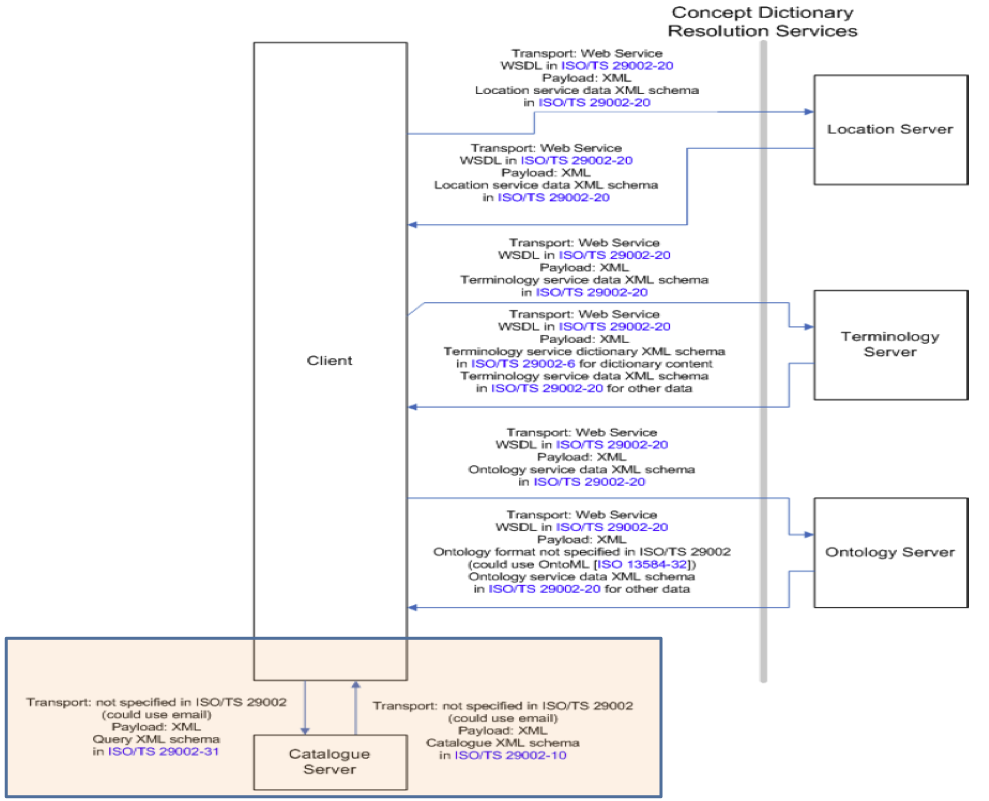
\includegraphics[width=0.99\textwidth]{images/datenfluesse_plib.png}
	\caption{Datenflüsse}
	\label{fig:datenfluesse}
\end{figure}
xxx Quelle???

% TODO was passiert bei langläufigen Abfragen? z.B. kaskadiert wie in einer Präsentation, wo der Anbieter weiteren Subanbietern einen Query schicken muss? Idee? Lösung? Asynchron im Web?

